\section{Genesis of the Project}

\subsection{The Need for Software Assurance}

\begin{center}
    \emph{``Software is eating the world.''\\}
    - Marc Andreessen
\end{center}

Nowadays, software is not just making things better as an ingredient. More and more services we consume are actually made up mostly or entirely of software. Even our most critical infrastructures now heavily rely on software: air traffic, self-driving vehicles, power plants, etc. We put our trust in software in our everyday lives, but how reasonable is this?

No software can be considered bug free. Written by humans, some errors are quickly discovered, whilst others may lie in wait for months and even years before being discovered by either a certain situation or the dedicated efforts of hackers. The more elaborate the system, the more complex and unavoidable the security defects. Any program, no matter how innocuous it seems, can harbor security holes. Thus, we should consider any software guilty until proven innocent \cite{cheswick2003firewalls}. Software assurance is not to be dealt with lightly, because a single defect in the code can lead to dreadful consequences. Think about how a single integer overflow resulted in the explosion of the first Ariane 5 space rocket, shutting down months of development in a matter of 37 seconds.

Gone are the days when our focus could lie solely on the functional aspects of software, because the source code would only be executed by ourselves in a controlled and safe environment. Facing the growth of distributed IT systems over the Internet, software assurance became a vital requirement.

``Historically, the symptoms of bad software security have been treated as a field problem to be solved with firewalls, application firewalls, intrusion detection systems, and penetration testing'' \cite{chess2007secure}. Focusing on security after the software is built is the wrong thing to do. It is like taking out the batteries of a smoke detector instead of trying to find the fire; it simply does not work at all. Figure \ref{fig:treating-the-symptom} illustrates this late-in-game approach.

\begin{figure}[ht]
  \centering
  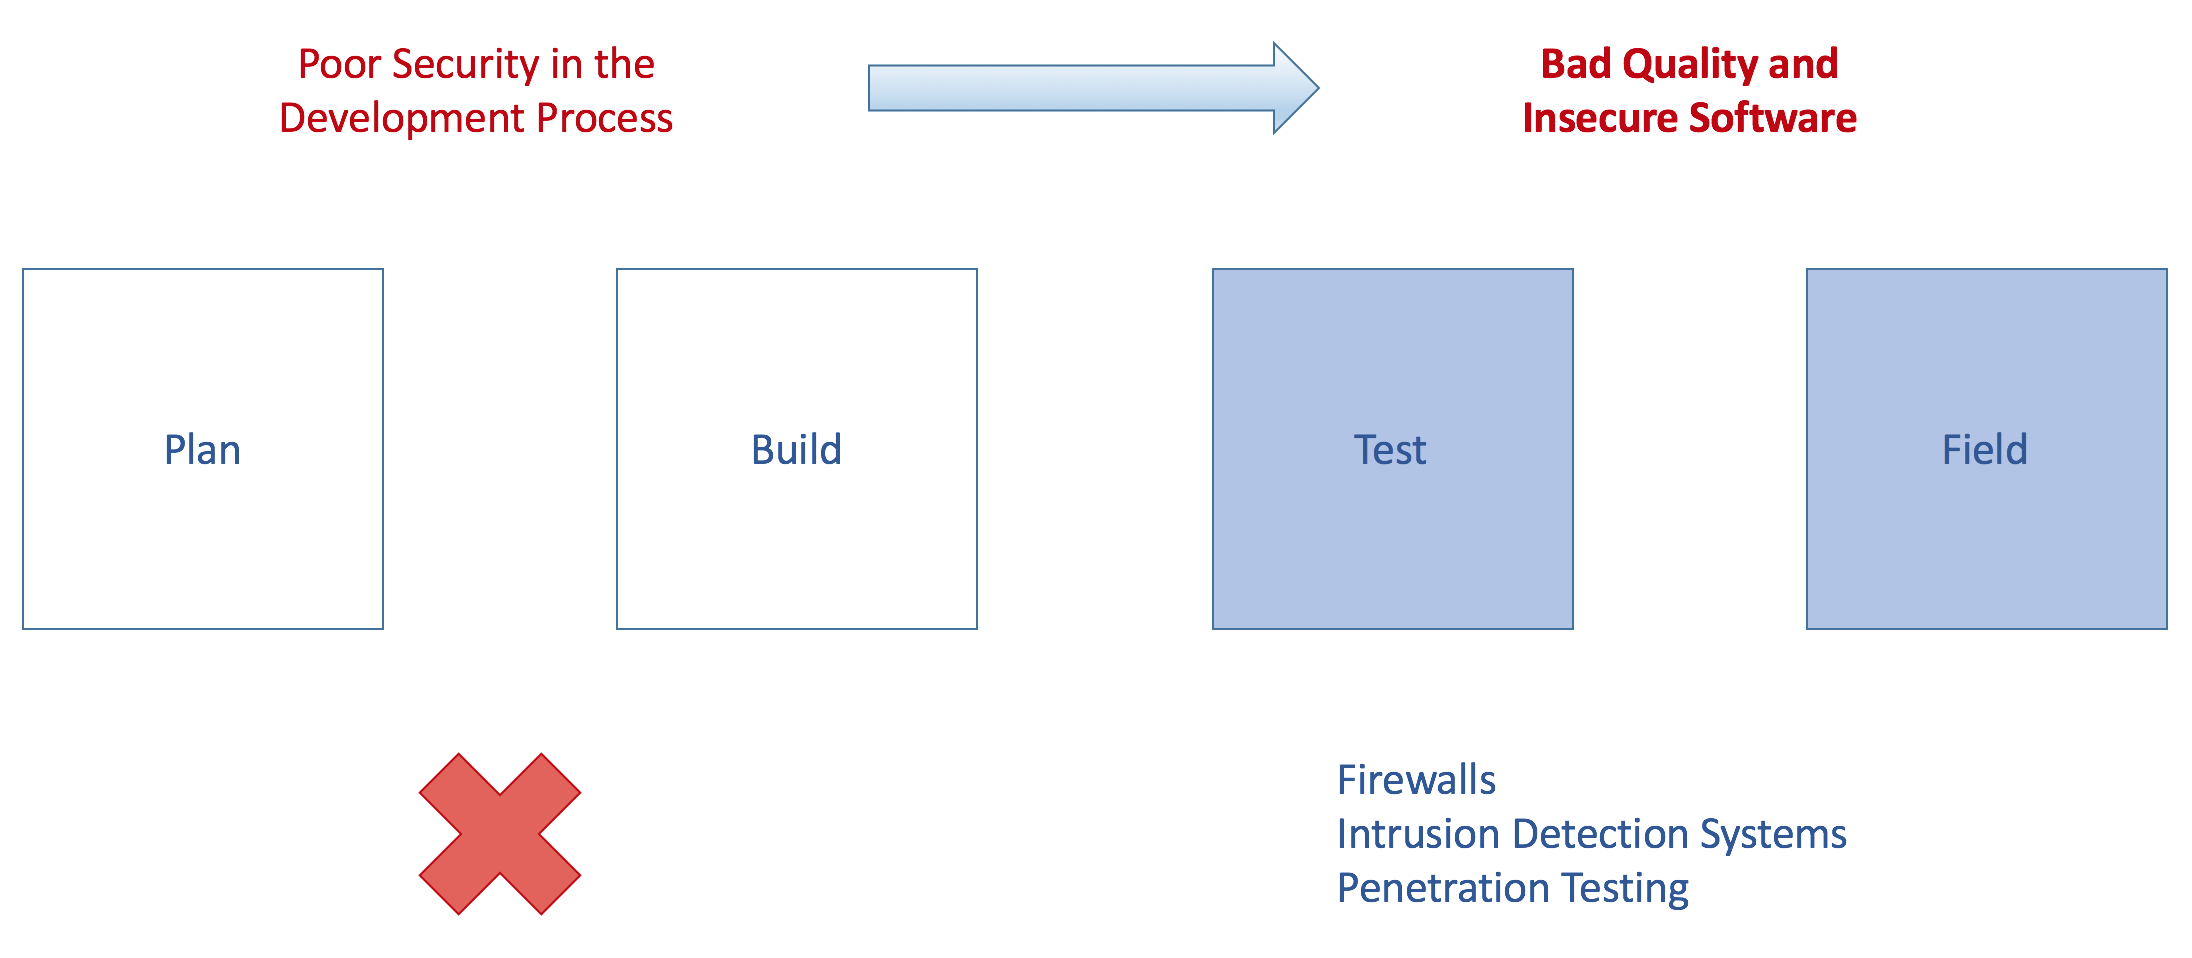
\includegraphics[scale=0.41]{figures/treating-the-symptom}
  \caption{Treating the Symptom (modified from \cite{chess2007secure})}
  \label{fig:treating-the-symptom}
\end{figure}

New software should be error free and secure. It must be developed to have high quality in the first place and be regularly maintained. Security should be an integral part of the development process: this way we can focus on the cause of most software security problems, the software itself (see Figure \ref{fig:treating-the-cause}). We are not saying that security should stop to be part of testing and fielding software, it should continue, but with a diminished emphasis \cite{chess2007secure}.

\begin{figure}[ht]
  \centering
  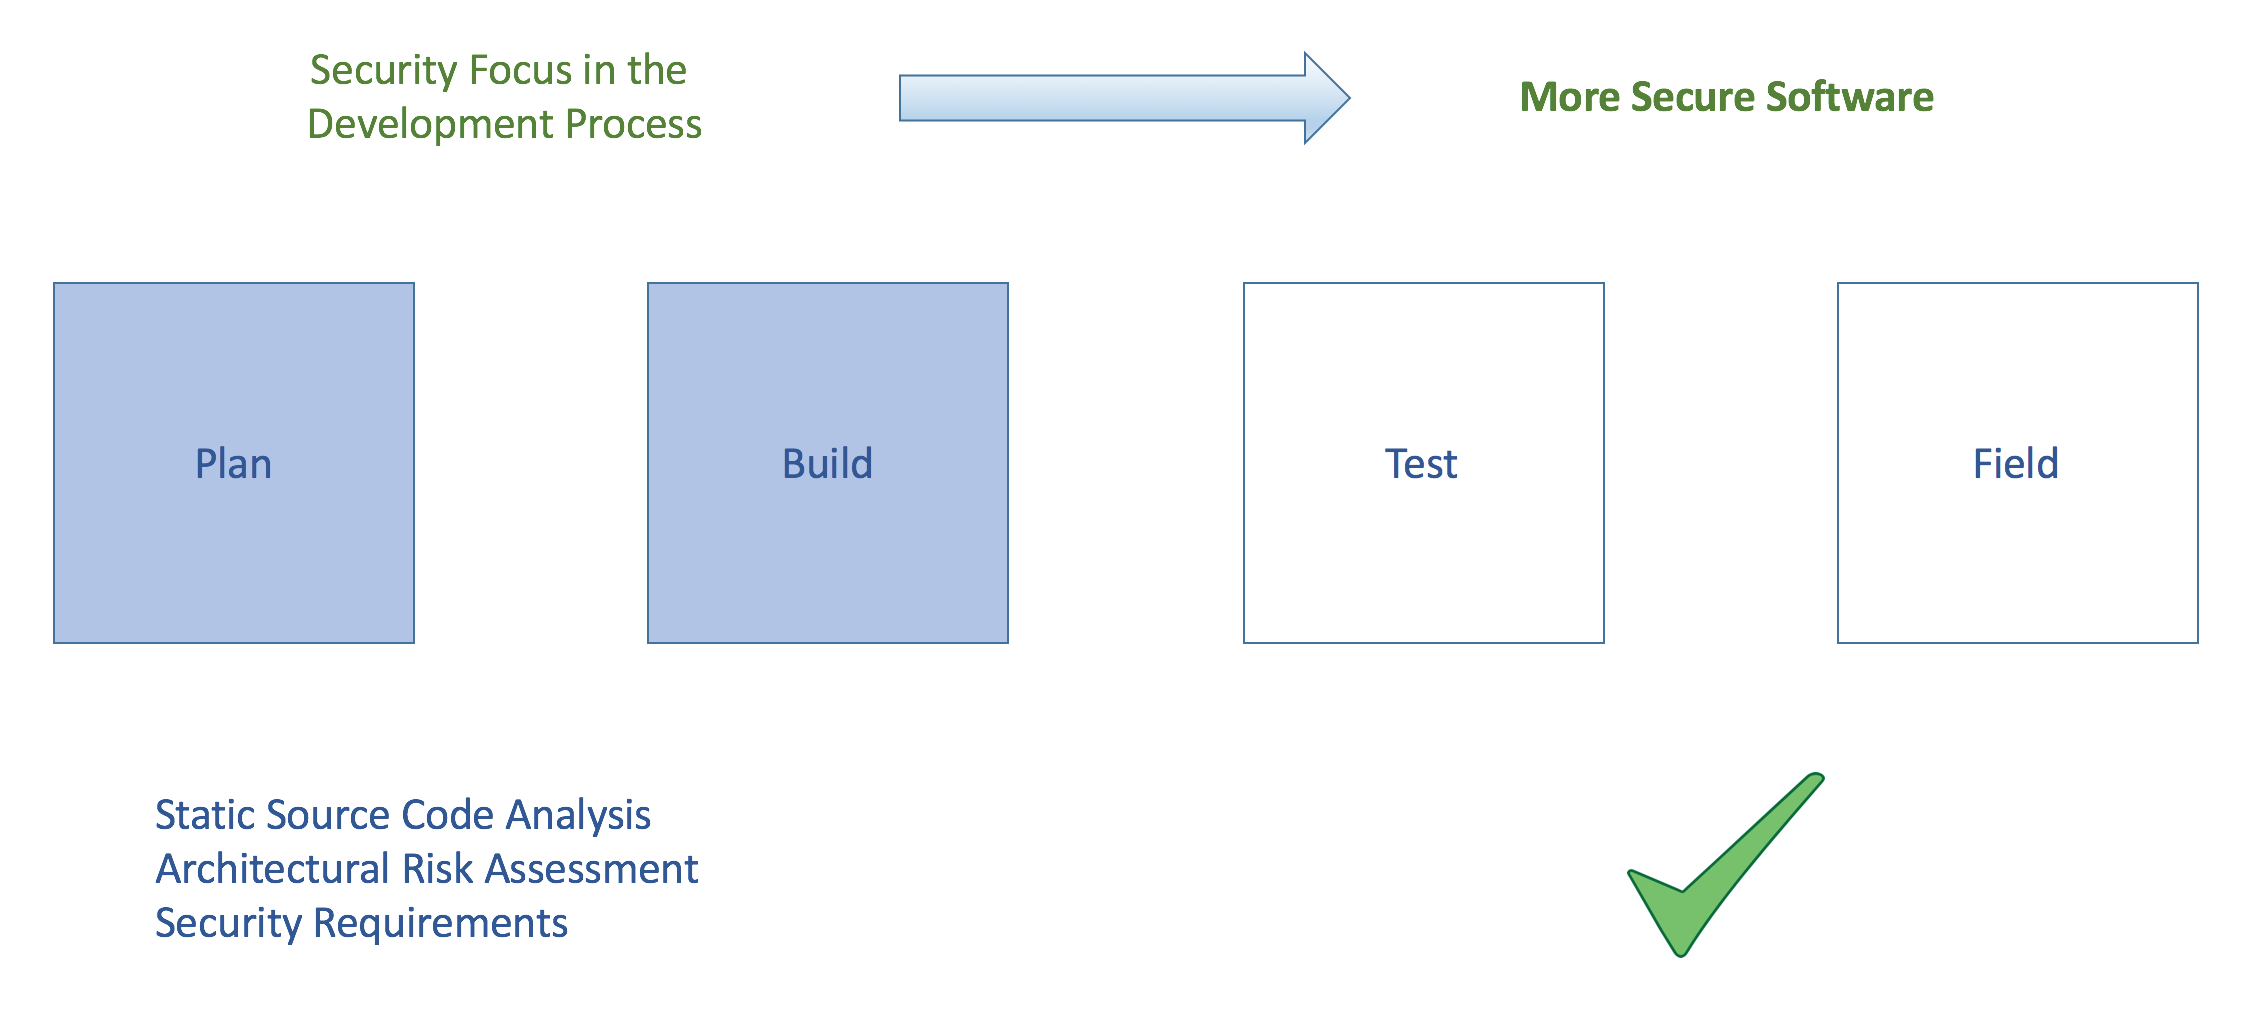
\includegraphics[scale=0.41]{figures/treating-the-cause}
  \caption{Treating the Cause (modified from \cite{chess2007secure})}
  \label{fig:treating-the-cause}
\end{figure}

The real question is: how can we prevent our software from being tainted with bugs? How can we assure our code is going to run the way it is intended to?

\clearpage

\subsection{Static Analysis: a Glimpse of Hope for Software Assurance?}

\vspace{1cm}

Good development methods and consistent testing are surely a first step to build secure code. Most of the time, however, it is not enough to deal with the countless execution paths that exist in large, realistic production software. Moreover, security problems also grow out of a lack of understanding about what secure programming entails: programmers are often completely unaware of the various ways an attacker could try to take advantage of a piece of code \cite{chess2007secure}.

\vspace{0.3cm}

For almost as long as computer programs have existed, many automated techniques \cite{nist2016classes} have been proposed to tackle security issues before they grew and were exploited. Those techniques fall into two main categories: dynamic and static analyses\footnote{~We will give a more thorough and accurate definition of Static Analysis and Dynamic Analysis in Section \ref{sec:static-analysis}}. ``Static and dynamic analyses arose from different communities and evolved along parallel but separate tracks. \dots{} Static analysis examines program code and reasons over all possible behaviors that might arise at run time. Compiler optimizations are standard static analyses. \dots{} Dynamic analysis operates by executing a program and observing the executions. Testing and profiling are a [\emph{sic}] standard dynamic analyses'' \cite{ernst2003static}.

\vspace{0.3cm}

While both dynamic and static analyses exhibit their own strengths and limitations (which we will discuss later in Section \ref{sec:static-analysis}), the \gls{samate} team chose to focus more on static analysis. The reason why lies in the fact that static analysis has the potential to be complete and sound\footnote{~A sound tool will never report false claims, i.e., never suffers a false positive. When a warning is reported you can be sure there is a problem. It does not mean, though, that the tool will catch every defect in the code.} and work as a proof of correctness, whereas the results of dynamic analysis may not generalize to future executions. It is not possible to ensure that the test suite chosen as input for a dynamic analysis is characteristic of all possible program executions.

\vspace{0.3cm}

Thus, by the mid-2000s, static analysis arose as a powerful approach to avoid or remove source code defects before they would actually be triggered or exploited. Static analysis not only gets rid of any of the bias a programmer could have regarding a piece of code, but it can often point to the root of a security problem, not just one of its symptoms. The IT community witnessed the birth of sophisticated static analysis tools, also known as static analyzers, dreaming that those tools would automate the code review process and help produce bug free software.

\vspace{0.3cm}

However, static analysis is a complex and computationally undecidable problem. Therefore, static analysis tools are not perfect and produce many unexpected and inaccurate results, also known as false positives and false negatives. Furthermore, running static analysis on large software remains a time/memory resource intensive process. The need to assess the effectiveness of those tools to understand how they work, and how much work and time they effectively save during the code review process became apparent.

\subsection[Assessing Static Analyzers]{Assessing Static Analyzers: Challenges of Producing Vulnerability Corpora}

\vspace{1cm}

For the last 25 years, automating \gls{vulnerability} discovery in software has been a major research and industry goal. However, evaluation has always been challenging. Ideally, the way to study the effectiveness of bug-finding tools, is to run them on large existing production software and analyze their output. But this vision has been hampered by the lack of proper \gls{vulnerability} corpora, with which to evaluate tools and techniques.

\vspace{0.3cm}

In fact, \gls{vulnerability} corpora do exist, but they are of limited utility and quantity \cite{kass2005nist}. To draw the most valuable and reliable conclusions from static analysis evaluation, the test material must exhibit three characteristics \cite{delaitre2013massive,delaitre2015evaluating}:

\vspace{0.3cm}

\begin{description}
    \item [\emph{Relevance}] Ultimately, static analyzers are designed to run on production software. Real software tends to be very complex with intricate control and data flows, whereas synthetic test material usually fails to provide such convoluted structures. Whilst a tool may perform well on crafted test data, it still might operate poorly on real software. In order to compute meaningful metrics from an evaluation, the test data should be representative of real software, i.e., used in production environments and developed according to industry standards.
    \item [\emph{Statistical Significance}] Because a small code base will feature a limited number and diversity of defects, the results would not demonstrate all of the capabilities of the tools studied. It might even lead to erroneous conclusions: a tool could score perfectly when finding a unique \gls{weakness} of a particular type. It would be ranked poorly if it overlooked another unique \gls{weakness} of the code base, even if it usually performed well at finding this type of \gls{vulnerability}. To yield statistical significance, the test suite should be large enough to contain many occurences of the same defect types along with a wide \gls{weakness}-type diversity.
    \item [\emph{Ground truth}] Finally, for assessing tool warnings, knowledge of where all bugs are located in the source code---a.k.a.\ ground truth---is required. Testing the behavior of static analyzers on test cases with clearly identified \glspl{weakness} helps deducing which \glspl{weakness} remain undetected and computing other relevant metrics.
\end{description}

\vspace{0.3cm}

Consequently, ideal test cases would be a set of large production software, developed according to industry standards, with well annotated and identified bugs embedded in the source code. Since those are out of reach, or would imply a gargantuan work to produce, evaluating static analyzers is definitely an intriguing topic.

\clearpage

\subsection{Static Analysis Tool Exposition (SATE)}

\vspace{0.5cm}

\subsubsection{What is \gls{sate}?}

\vspace{0.5cm}

\begin{flushright}
    \emph{``Never give up on a dream just because of the time it will take to accomplish it.\\ The time will pass anyway.''\\}
    - Earl Nightingale
\end{flushright}

However impossible it seems to produce completely safe and secure software, the NIST \gls{samate} project is deeply committed to raising the quality of industrial software and providing the community with best practices for secure software development.

To address the need of assessing the effectiveness of static analyzers, the \gls{samate} project conducted the first Static Analysis Tool Exposition (\gls{sate}) in 2008. In total, \gls{samate} has organized five editions of \gls{sate}, the last one being \gls{sate} V held in March 2014. These expositions were designed to advance research in static analysis tools that find security-relevant defects in source code. \gls{sate} has these goals:

\begin{itemize}
    \item To enable empirical research based on large test sets
    \item To encourage improvements of tools
    \item To speed adoption of the tools by objectively demonstrating their use on production software
\end{itemize}

For each edition of \gls{sate}, \gls{samate} provided participating tool makers with a set of programs also called test cases. The tool vendors ran their static analyzers on the provided test sets and produced complete reports. Those reports were further processed by NIST researchers and the results were reported during a workshop \cite{okun2010second,okun2011report,okun2013report,okun2009static,okun2016sate}.

\vspace{0.5cm}

\subsubsection{\gls{sate}'s Test Material}

\vspace{0.5cm}

Over its five instances, \gls{sate} has been refined to provide more accurate conclusions on static analysis tools. Notably, \gls{samate} has designed a solution to address the lack of appropriate \gls{vulnerability} corpora.

As we have seen before, no candidate \gls{vulnerability} corpora exhibits the three aforementioned characteristics: relevance, ground-truth, and statistical significance. However, test cases exhibiting any two of the three characteristics are readily available:

\clearpage

\begin{description}
    \item[Production Software] Production software is germane by definition. It is large enough to achie\-ve statistical significance, but the defects are only partially known and finding all of them is impractical with the current state of the art. Ground-truth is, therefore, unreachable for production software.
    \item[The \glspl{cve} \cite{mitre2016cve}] CVEs is the most prominent effort to  provide the IT community with a database of publicly disclosed \glspl{vulnerability} in production software. Cataloging real software containing known \glspl{vulnerability}, CVEs form a good candidate for ground-truth and relevance. But there are just simply not enough examples for statistical significance.
    \item[Synthetic Test Cases] Synthetic Test Cases are programs developed with computer assistance to incorporate a particular \gls{vulnerability}. These programs are usually small and can be artificially produced in great numbers. Among these synthetic corpora, the Juliet test suite is the most prominent effort to this day with more than 60k C/C++ test cases and 25k Java test cases \cite{nsa2016juliet}. Ground truth and statistical significance are provided by definition, but the \glspl{vulnerability} might not be embedded into realistic control flow and data flow structures. Accordingly, synthetic test cases may not represent the relevant properties of software.
\end{description}

By combining the 3 types of test cases described above, it is, therefore, possible to study the behavior of static analyzers in a complete way (Figure \ref{fig:types-of-test-cases}). This solution might not be ideal, but this is the closest we can get to understanding the tools' behavior in a production environment. It is at least possible then to compute useful metrics to evaluate the performance of static analyzers.

\vspace{1.5cm}

\begin{figure}[ht]
    \centering
    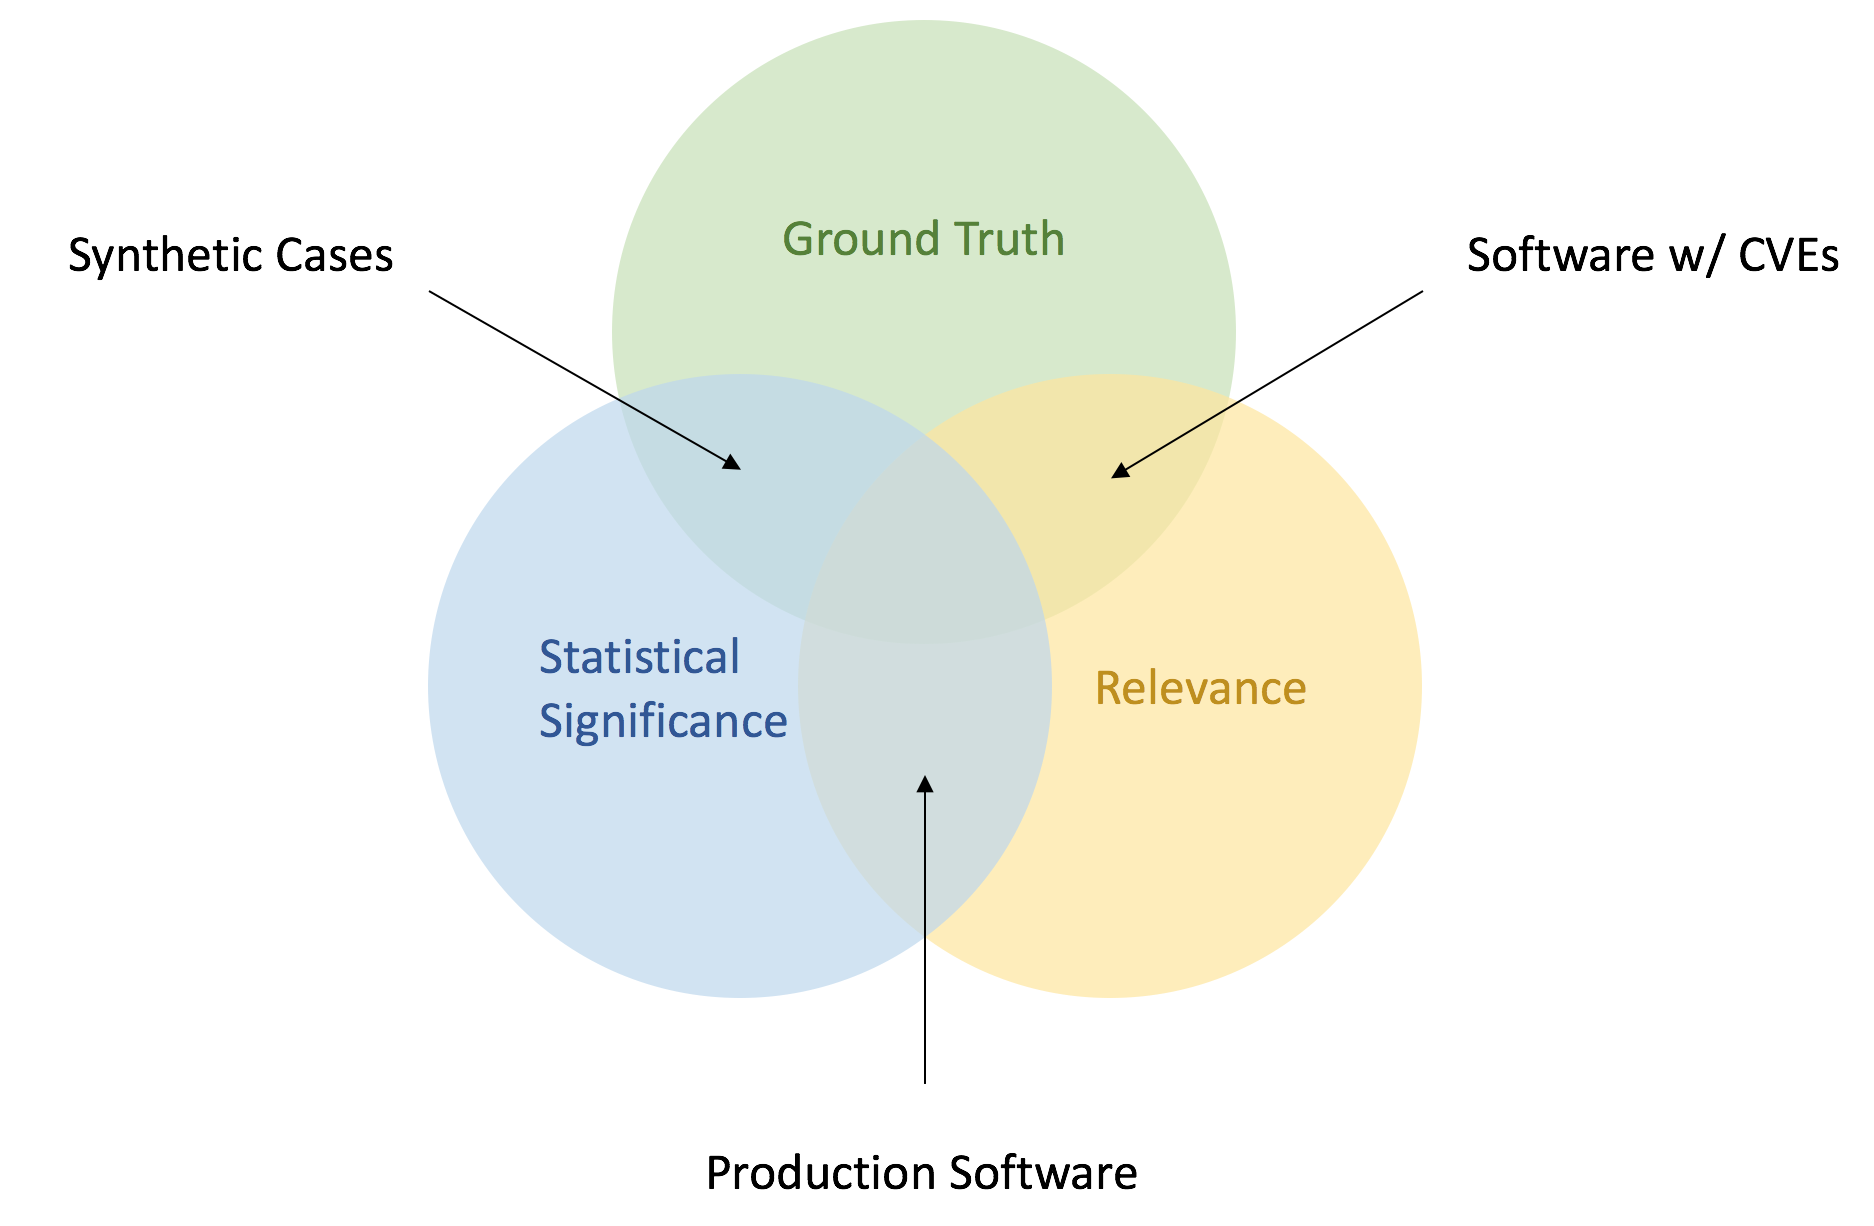
\includegraphics[scale=0.49]{figures/types-of-test-cases}
    \caption{\gls{sate} Types of Test Cases \cite{okun2016sate}}
    \label{fig:types-of-test-cases}
\end{figure}